\documentclass[10pt, letterpaper]{article}
        \usepackage[utf8]{inputenc}
        \usepackage[margin=1in]{geometry}
        \usepackage{fancyhdr}
        \usepackage{titling}
        \usepackage{enumitem}
        \usepackage{mathtools}
        \usepackage{amssymb}
        \usepackage{xfrac}
        \usepackage{booktabs}
        \usepackage{graphicx}
        \usepackage{wrapfig, blindtext}
        \usepackage{hyperref}
        \usepackage{enumerate}
        \usepackage{multicol}

        
        \setlength{\parindent}{0pt}

\title{Journal 2}
        \author{Sudhan Chitgopkar}
        \date{\today}
        
        % headers -- no need to change
        \pagestyle{fancy}
        \fancyhf{}
        \lhead{GA 3}
        \chead{UGAMUNC XXVII}
        \rhead{\thedate}


\begin{document}

Dear Delegates,\\

It is with great pleasure that we welcome you to the third General
Assembly, the Social, Humanitarian, and Cultural Committee (SOCHUM) at
UGA's 27th Model United Nations Conference. My co-chair Sydney and I are
looking forward to a weekend full of fabulous and informed debates. My
name is Catherine Shih (she), and I will be your Chair. I am a
first-year intended International Business and Marketing major from
Johns Creek, Georgia. In addition to Model UN, I am involved in the
Atlas Business Society. In my free time, I enjoy watching cooking
videos, finding good music, and discovering new ways to make life more
interesting. I have been involved in Model United Nations throughout all
four years of high school, from leading our club to traveling the
country and attending conferences. In fact, Sydney and I competed
against each other at UGAMUNC her senior year of high school. Although I
am not pursuing a major directly related to MUN, it has certainly helped
me grow as a speaker and person and continues to teach me new things
everyday. \\

My co-chair this year is Sydney Thornton. Sydney is a second year
Anthropology student with a minor in Japanese and is pursuing two
certificates, one in sustainability and the other in Global Studies.
Sydney enjoys teaching outdoor skills, having been a volunteer with the
Boy Scouts of America and Girl Scouts of the United States for over ten
years. In addition to the Model UN team, Sydney is the historian for
UGA's Alpha Lambda Delta Chapter, volunteers at the UGArden, and helps
out at many community events. In her free time, when she has it, she
loves to travel and write her own fictional stories. She is just as
excited as I am to help chair this committee and hear all of your
wonderful solutions to these important issues! \\

We invite you to read this background guide and develop a plan that will
best showcase your abilities at this conference. Please be respectful as
these topics contain sensitive issues. Compete in this committee with
integrity and approach these topics with an open mind and be ready to
have some fun! \\

In regards to position papers, please focus your research within the
scope of your country and maintain that focus during the committee. Your
work and speeches should align with your country's ideals. The
resolutions drafted should reflect the work of SOCHUM and its mission.
We will review parliamentary procedure with you at the beginning of the
conference but we implore you to look through the UGAMUNC rules on our
website, 
\texttt{\href{https://www.ugamunc.com/}{{https://www.ugamunc.com/}}},
especially given our new changes in regards to COVID. My email is
\texttt{\href{mailto:catherineshih@uga.edu}{{catherineshih@uga.edu}}}
if you need my help. Please email your position papers to Sydney at
\texttt{\href{mailto:smt12493@uga.edu}{{smt12493@uga.edu}}} \textbf{by February
1 at 11:59 PM.} Come prepared, do your research, and get ready for an
awesome weekend! \\

We can't wait to see you in committee! Sincerely,

Catherine Shih and Sydney Thornton

\newpage
\tableofcontents
\newpage

\section{{An Introduction to SOCHUM}}

The Third General Assembly of the United Nations aims to address social,
humanitarian, and cultural issues (SOCHUM). This committee ``discusses
questions relating to the advancement of women, the protection of
children, indigenous issues, the treatment of refugees, the promotion of
fundamental freedoms through the elimination of racism and racial
discrimination, and the right to self- determination on the behalf of
the United Nations. Conflicts that involve political manners are meant
to be addressed by the Fourth General Assembly, which was created to
address Special Political and Decolonization issues (SPECPOL).
Therefore, our committee cannot deal with political matters. Our
resolutions must cover the result of these issues, not their political
roots. For example, Topic 2 of this committee addresses the right to
protest and whether governments are humanly treating those who use their
right to freedom of speech, not the political events that started these
protests. You must keep in mind the abilities of this committee as the
conference moves forward. \\

Human rights are the core of this committee. Many of these rights
correspond with the United Nations Human Rights Council (UNHCR). This
council was established by the General Assembly in 2006 in order to
affirm human rights and bring violations to the global stage. Our basic
rights are something that need to be protected and the rights of others
must be defended. \\

This assembly believes that the rights of the disparished need to be
focused on. The topics of this committee deal with sensitive issues like
unequal access to healthcare, systemic racism, trafficking and abuse,
and more. While these are contentious topics, it is important to
remember that this assembly has created numerous resolutions that have
helped people facing these issues and more. This assembly has helped
millions of people with its work and will continue to do so in an ever
tumultuous world. \\

We now invite you to step in and immerse yourself in the third General
Assembly. As a delegate, you have the ability to create legislation that
will solve some of the most pressing global issues on the planet. We
expect respectfulness, class, professionalism, and an open mind in
regard to finding appropriate solutions. In a world rapidly facing
change, we encourage you to embrace that change and bring about positive
ideas to make the world a better place. \\

This committee covers a wide range of issues. Some of these issues have
never been seen prior to the emergence of the COVID-19 pandemic. But
with this background guide, you are expected to take your country's
stance on these issues plaguing our world. Take into the account the
abilities of SOCHUM and develop a plan of attack to cover all sides of
these issues. We look forward to seeing your debate and the solutions
you bring to the table. \\

\newpage
\section{{Topic A: Destigmatizing Mental Health across the
globe}}

\subsection{Introduction:}

\begin{wrapfigure} {r} {0pt}
\centering
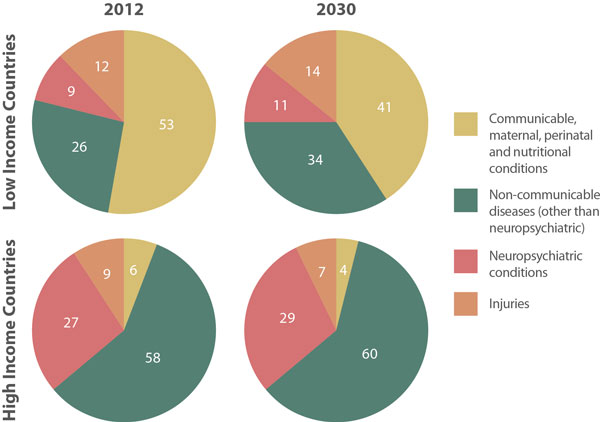
\includegraphics[scale = 0.4]{image1.jpg}
\end{wrapfigure}

Mental health is a relatively new topic to be discussed on a global
scale. Most people who live their entire lives with mental illness have
been blamed for their condition and often told that they can control
their mental illness. Many people are often discriminated against and
deprived of justice. One of the largest issues that we hope to see
resolved within this committee is dissolving negative stigma which
prevents people from seeking the help they need as well as gaining a
route to living a normalized life in which they are treated fairly.
Additionally, within many nations, mental health services are
insufficient and limited options force many people to turn to
alternative coping methods such as drugs in order to alleviate the pain
they feel from their mental health. \\

Within middle income countries and low income countries we see how
health systems lack access to high-quality mental health services.
Stigma, human resource shortages, lack of research, and inadequate
service delivery models all contribute to a mental health treatment gap
within these nations. We hope to see how nations will come together and
collaborate in resolving this issue. \\

\subsection{Background Information}

  \begin{wrapfigure}{l}{0pt}
\centering
    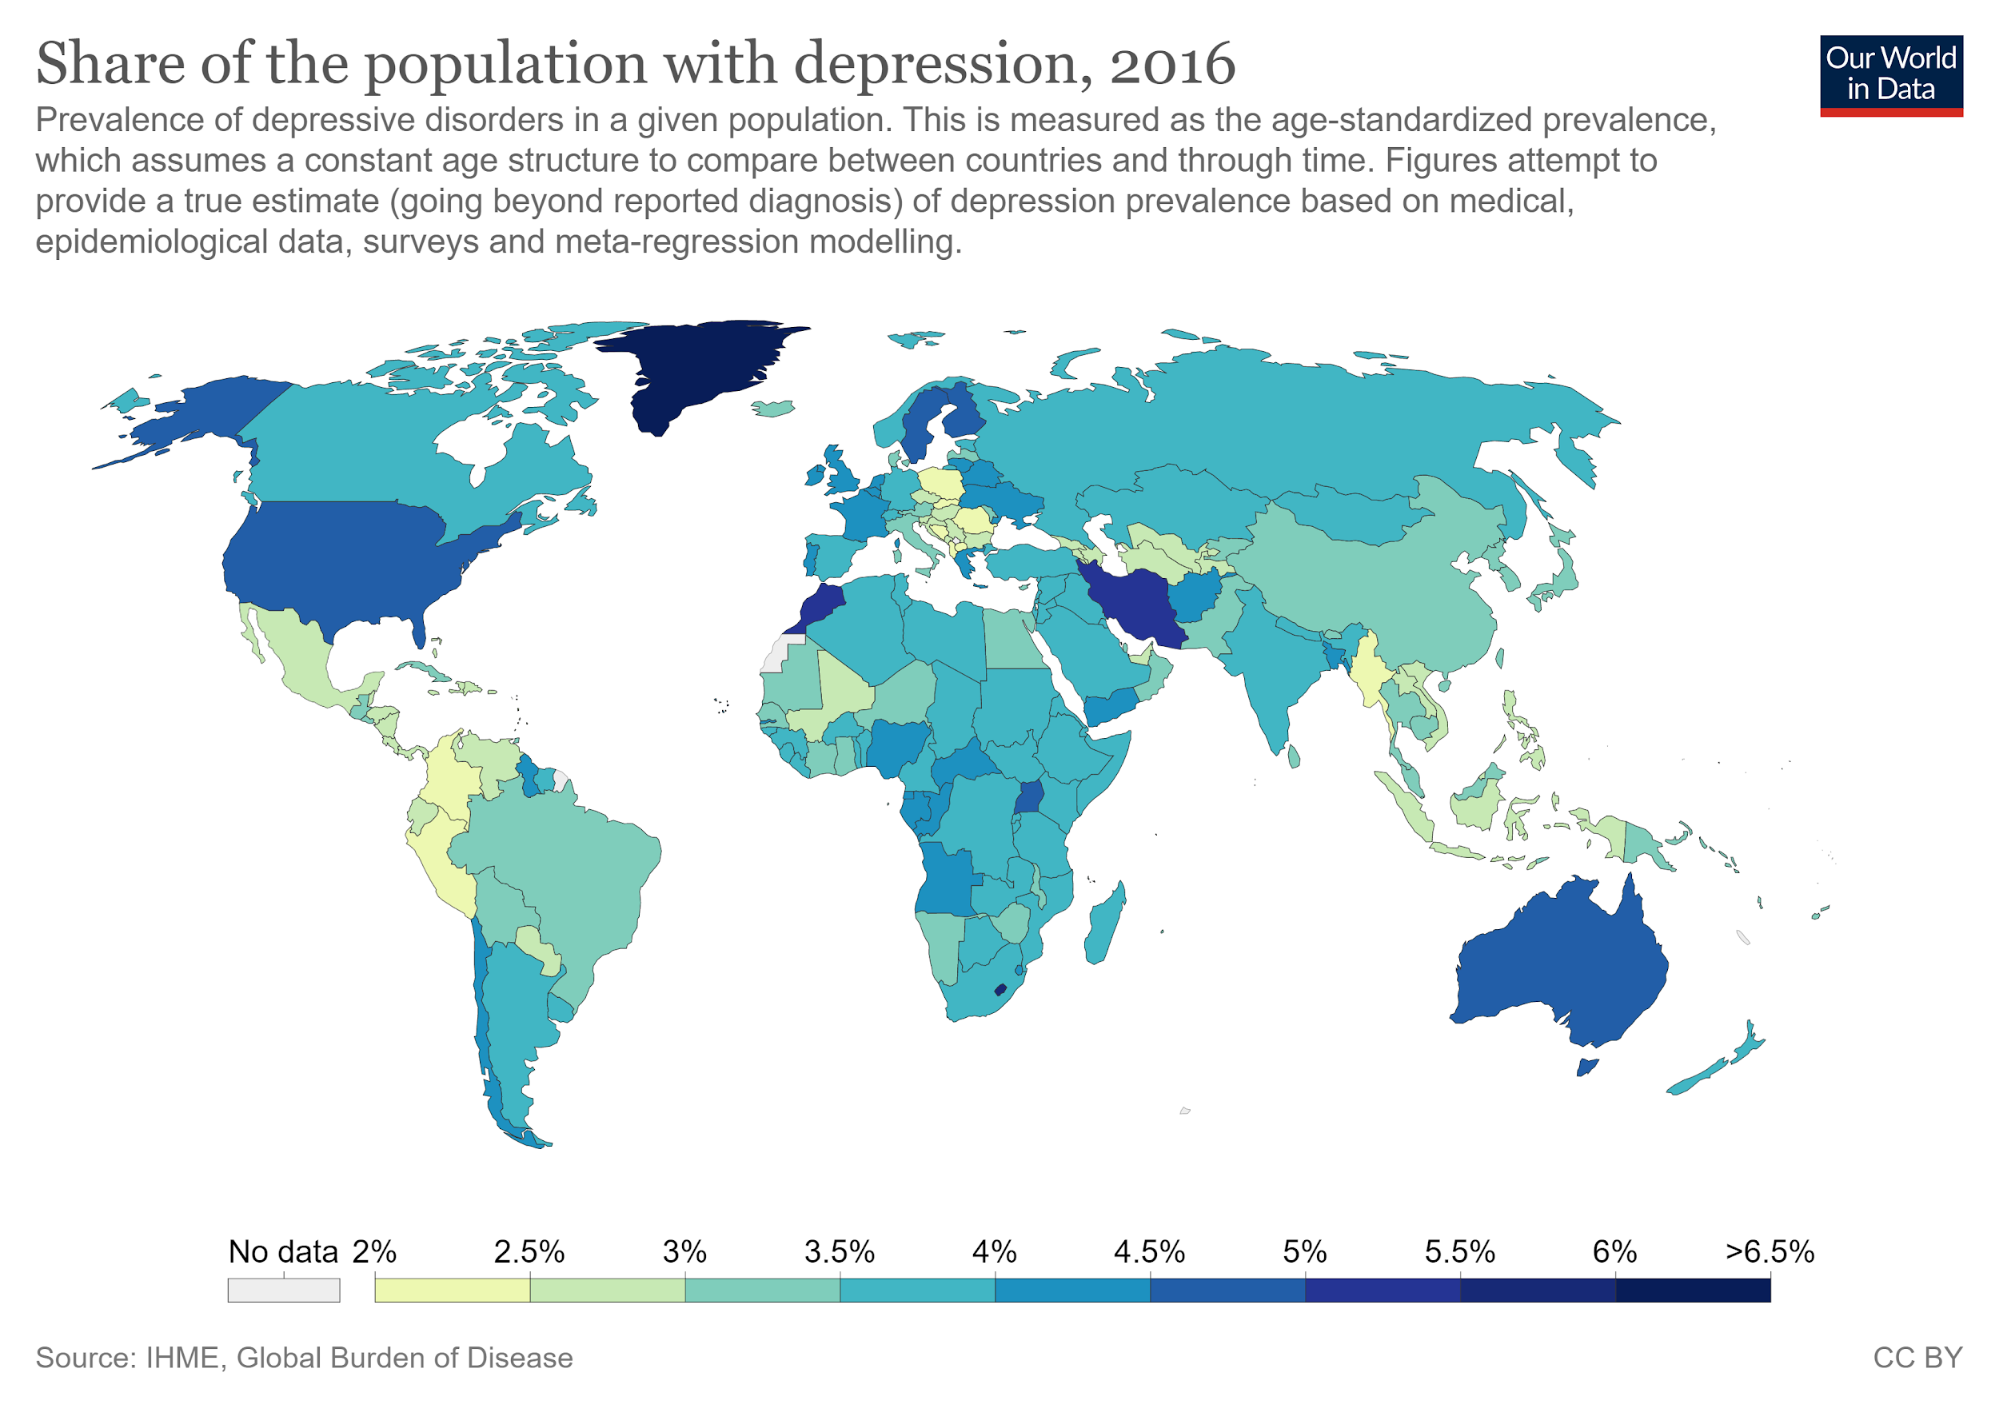
\includegraphics[scale= 0.1]{image2.png}
    \caption{2016 Global Depression Rates.\footnote{Ritchie,
  Hannah, and Max Roser. ``Mental Health.'' Our World in Data, January
  20, 2018. https://ourworldindata.org/mental-health.}}
\end{wrapfigure} 

The World Health Assembly adopted the comprehensive mental health action
plan for the years of 2013 to 2020. This committed United Nations member
states to provide mental health care that will be integrated into
primary care for both common and severe mental disorders. Additionally,
the United Kingdom Department for International Development created an
assortment of both research institutions and ministries of health in
five of LMICs in Ethiopia, India, Nepal, South Africa, and
Uganda\footnote{9 Ways to Fight Mental Health Stigma. (n.d.). Retrieved
  October 21, 2020, from
  https://www.nami.org/blogs/nami-blog/october-2017/9-ways-to-fight-mental-health-stigma}.
These are a prime example of creating different evaluation and cost
measurement methodologies for integrating mental health into healthcare
context, as many of these nations are working towards utilizing modern
technologies into their healthcare systems. Many of the best practices
that are being used around the world have been identified through these
different organizations and used to customize mental health services
into the system. Additionally multiple studies with NHIC's indicate that
mental disorders are more effectively treated using different forms of
testing, however, that's forms of testing are relatively expensive and
difficult to implement in all nations.\footnote{Wainberg, M., Scorza,
  P., Shultz, J., Helpman, L., Mootz, J., Johnson, K., . . . Arbuckle,
  M. (2017, May). Challenges and Opportunities in Global Mental Health:
  A Research-to-Practice Perspective. Retrieved October 21, 2020, from
  https://www.ncbi.nlm.nih.gov/pmc/articles/PMC5553319/} \\

The world health organization has created a world mental health day
which is observed on October 10 every year. This is the day that
provides an opportunity for all people working within the mental health
sphere to talk about their work and share more scientific research done
in relation to mental health. Mental health is one of the most neglected
areas of public health. And now due to the issues of the COVID-19
pandemic, many have suffered more from their mental health as many are
stuck in their homes and unable to leave. More than 75\% of people with
mental disorders or substance use disorders receive no treatment due to
the fact that they are unable to meet their therapist or health care
provider face-to-face. On average countries spend only 2\% of their
health budgets on mental health. However many nations do not know that
when there is an increase in development assistance for mental health,
and more investment in treatment for mental disorders, there is a return
in improved health and productivity within the workplace. Discovering
the relations between improved mental health and the economy will
further create conversation within how investing in the mental health
industry will provide opportunities for people around the world to be
encouraged to join the workforce and share their own experiences with
mental health. 

\subsection{Vocabulary:}
\begin{itemize}
\item     
\textbf{Mental Health:} the psychological state of someone who is
functioning at a satisfactory level of emotional and behavioral
adjustment
\item 
\textbf{Clinical Social Worker:} Provides mental health services for the
prevention, diagnosis, and treatment of mental, emotional, and
behavioral disorders in individuals, families, and groups.
\item 
\textbf{Underinvestment:} a situation in which less money is spent on
something over a long period of time than is needed.
\item 
\textbf{Social Stigma}: Social stigma is the disapproval of, or
discrimination against, a person based on perceivable social
characteristics that serve to distinguish them from other members of a
society.
\end{itemize}

\subsection{Questions to Consider:}

\begin{itemize}
\item
  
  How will this committee provide access to mental health resources?
  
\item
  
  How will cultural stigmas in regard to mental health be addressed?
  
\item
  
  How will people be protected in cultures that demonize mental health?
  
\item
  
  How will education be provided in regard to different mental illnesses
  and disorders and what incentives, if any, should be looked into?
  
\end{itemize}

\newpage
\section{{Topic B: The Protection Over the Right to Protest}}

\subsection{Introduction:}

In 2020, many countries have seen protests arise over a number of
different issues. School children protesting climate changes, calls for
recounts in seemingly illegitimate elections, and outcries for police
reform. Almost every continent has had some sort of major protest that
received global attention this year. Tear gas, arrests, beatings, and
more have marked these outcries for change. \\

In a world that's facing more and more trouble each day, it calls into
question whether or not the right to free speech is globally ensured.
Article 19 of the Universal Declaration of Human Rights states that
``everyone has the right to freedom of opinion and
expression\footnote{``Universal Declaration of Human Rights.'' United
  Nations. United Nations, n.d.
  https://www.un.org/en/universal-declaration-human-rights/.}.'' As more
people are being harmed for their opinion, it begs the question ``what
protects free speech?'' \\

\subsection{Topic Background:}

The year started with protests that continued from 2019. For example, in
April 2019, the Chinese government introduced a bill to allow
extradition from Hong Kong to mainland China\footnote{``The Hong Kong
  Protests Explained in 100 and 500 Words.'' BBC News. BBC, November 28,
  2019. https://www.bbc.com/news/world-asia-china-49317695.}. While the
bill was withdrawn after protests first erupted, they continued and grew
more and more violent. Police first fired on protestors and used water
cannons to try and subdue protestors\footnote{Leung, Yan Zhao and
  Jasmine. ``Hong Kong Police Fire First Gunshot, Water Cannon in
  Protest Clashes.'' Yahoo! News. Yahoo!, August 25, 2019.
  https://news.yahoo.com/hong-kong-police-water-cannon-latest-clashes-113026680.html.}.
Things have not improved as protests grew larger and larger, with pepper
spray being used on crowds that gathered on the one year anniversary of
the protests beginning\footnote{``Pepper Spray Used as Hundreds Gather
  in Downtown Hong Kong.'' South China Morning Post, June 10, 2020.
  https://www.scmp.com/news/hong-kong/politics/article/3088249/hong-kong-protests-hundreds-gather-central-mark-first.}. \\

The original contention of these protests were over China's overstep in
governmental policy. Hong Kong was originally a British colony that was
handed to the Chinese government under the notion that they would still
be able to have their own judicial and legal system. Many counties have
called into question whether that system has been maintained, with the
US revoking Hong Kong's ``special status,'' an action that brought about
Chinese threat\footnote{Zhang, Zoey. ``US Revokes Hong Kong's Special
  Status: What Are the Implications?'' China Briefing News, August 14,
  2020.
  https://www.china-briefing.com/news/us-revokes-hong-kongs-special-status-implications-trade-business/.}. \\

\begin{wrapfigure} {r} {0pt}
\centering
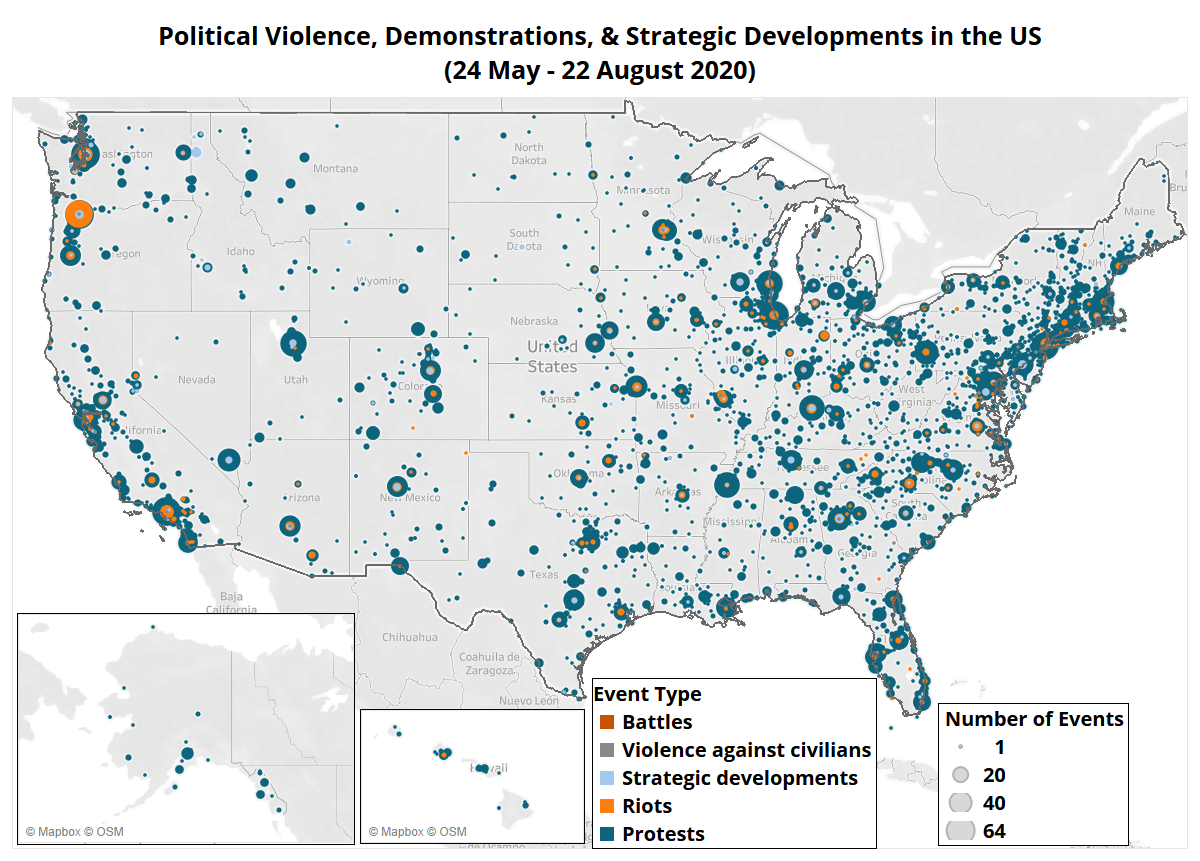
\includegraphics[scale = 0.2]{image5.png}
\caption{Protests \& calls for change\footnote{Author:
  Roudabeh KishiRoudabeh Kishi is the Director of Research \& Innovation
  at ACLED. She oversees the quality. ``Demonstrations \& Political
  Violence in America: New Data for Summer 2020.'' ACLED, October 8,
  2020.
  https://acleddata.com/2020/09/03/demonstrations-political-violence-in-america-new-data-for-summer-2020/.}}
\end{wrapfigure}

Hong Kong is not the only part of the world experiencing protests about
police reform. Throughout 2020, the United States has been facing calls
for police reform in regards to the mistreatment of African American
citizens. The protests came as a result of the killings of Breonna
Taylor, Ahmaud Arbery, George Floyd, and many more. This sparked outcry
across the country, causing protests in an already pressured population
from the constraints of the COVID-19 pandemic. Similar to
the people of Hong Kong, protesters wanted police reform after being
systematically oppressed by the people in power. Tear gas\footnote{Al
  Jazeera. ``US Federal Agents Use Tear Gas to Disperse Portland's BLM
  Protest.'' US \& Canada \textbar{} Al Jazeera. Al Jazeera, July 25,
  2020.
  https://www.aljazeera.com/news/2020/7/25/us-federal-agents-use-tear-gas-to-disperse-portlands-blm-protest.},
rubber bullets, water cannons, and more were used by police on people
that were protesting peacefully. Some experts cite the rise in American
protests as the result of multiple social and political stressors. The
last few years have consisted of large amounts of mass
shootings\footnote{Silverstein, Jason. ``There Were More Mass Shootings
  than Days in 2019.'' CBS News. CBS Interactive, January 2, 2020.
  https://www.cbsnews.com/news/mass-shootings-2019-more-than-days-365/.},
rise in violent crimes\footnote{Al Jazeera. ``Hate Crime Violence in US
  Hit 16-Year High in 2018: FBI.'' US \& Canada \textbar{} Al Jazeera.
  Al Jazeera, November 14, 2019.
  https://www.aljazeera.com/news/2019/11/14/hate-crime-violence-in-us-hit-16-year-high-in-2018-fbi/.},
and more. The 2020 election was already on people's minds by spring
2020, resulting in high amounts of contention and stress amongst US
citizens. \\

Two of the most influential nations on the planet have had a year racked
with outcries and international concern over whether either truly uphold
the ideal of freedom of speech. With protestors in both nations being
brutally attacked, resulting in injuries on thousands of people, it
calls to question whether or not that right is being protected on a
global scale\footnote{Chan, Melissa. ``For Protesters Injured by Police,
  There's No Real Recovery.'' Time. Time, October 9, 2020.
  https://time.com/5894356/protesters-injured-police/.}. \\

\subsection{Other Global Movements:}

These two nations have not been the only ones to experience protests. In
fact, there have been many global movements occurring as people find
themselves fighting for what they believe in. \\

In August of 2018, Swedish activist Greta Thunberg began a strike on
going to school to advocate for climate change policies, hoping to bring
about change in a world rapidly being affected by climate
change\footnote{``Greta Thunberg.'' Encyclopædia Britannica.
  Encyclopædia Britannica, inc., September 8, 2020.
  https://www.britannica.com/biography/Greta-Thunberg.}. She soon began
gathering global attention, bringing about strikes across the world as
young people live in fear of what will happen to their planet. As of
September 2020, Thunberg has entered her 110th week of
protest\footnote{Harvey, Fiona. ``Young People Resume Global Climate
  Strikes Calling for Urgent Action.'' The Guardian. Guardian News and
  Media, September 25, 2020.
  https://www.theguardian.com/environment/2020/sep/25/young-people-resume-global-climate-strikes-calling-urgent-action-greta-thunberg.},
calling for students to strike from their now online classes and having
the support of notable businesses like Ben and Jerry's, Patagonia, and
more\footnote{Nguyen, Terry. ``Some Brands Are Closing Stores for the
  Global Climate Strike. That's a Big Deal.'' Vox. Vox, September 20,
  2019.
  https://www.vox.com/the-goods/2019/9/20/20876098/brands-global-climate-strike-closing.}.
Critics have said that Thunberg and the millions of her supporters are
too young to understand, which brings to question at what age one is
allowed to protest and have their views be considered valid. \\

In the wake of the COVID-19 pandemic, people across the world are being
forced to face a new reality. Mask mandates have been put out by
governments across the world, nasal swab testing is now a regular
procedure for most, and most aspects of a person's life have been moved
online. As a result, many have decided to voice their anger with this
new reality by using their right to protest. While the virus is not a
hoax, some believe the mandates to wear a mask violate their personal
freedoms, resulting in marches across the world. From the US\footnote{Beer,
  Tommy. ``Anti-Mask Rallies Continue In U.S. Amid Rising Coronavirus
  Cases And Deaths.'' Forbes. Forbes Magazine, July 16, 2020.
  https://www.forbes.com/sites/tommybeer/2020/07/16/anti-mask-rallies-continue-in-us-amid-rising-coronavirus-cases-and-deaths/.},
to Spain\footnote{``Coronavirus: Hundreds Gather in Madrid for Anti-Mask
  Protest.'' BBC News. BBC. Accessed October 20, 2020.
  https://www.bbc.com/news/av/world-europe-53802226.}, and more, people
have gathered around the idea that governments cannot force people into
quarantines or force them to wear masks as that violates their freedom
of choice as an individual. \\

\subsection{What does this mean?:}

In an increasingly divided world, we face the question of how well the
right to protest is protected. While people are allowed to disagree with
others and with government actions, when does someone's personal safety
become a common factor? When is someone allowed to protest and what is
done if that right is being violated? It has been witnessed across 2020
that some governments will not hesitate to harm its citizens. When the
UN can step in is up to the debate of this committee. \\

\subsection{Vocabulary:}
\begin{itemize}
\item
  
  \textbf{Special Status:} When a land or community is distinguished
  from a larger governing body.
  
\item
  
  \textbf{Climate Change:} A change in global temperature patterns as a
  result of human activity
  
\end{itemize}

\subsection{Questions to Consider:}

\begin{itemize}
\item
  
  To what degree can the UN protect an abstract concept like freedom of
  speech?
  
\item
  
  What efforts can countries take to protect their citizen's right to
  free speech?
  
\item
  
  How would these proposed solutions be monitored and enforced?
  
\item
  
  What if protests are against the government of a nation? How would the
  UN help without defying the governing body?
  
\item
  
  How does this right remain protected if it poses a threat to the
  health and safety of others?
  
\end{itemize}

\subsection{Suggested Readings:}

\begin{itemize}
\item
  
  \texttt{\href{https://www.bbc.com/news/world-asia-china-49317695}{{https://www.bbc.com/news/world-asia-china-49317695}}}
  
\item
  
  \texttt{\href{https://civilrights.findlaw.com/enforcing-your-civil-rights/is-there-a-right-to-peaceful-protest.html}{{\nolinkurl{https://civilrights.findlaw.com/enforcing-your-civil-rights/is-there-a-right-to-peaceful-protest.html}}}}
  
\item
  
  \texttt{\href{https://tulsaworld.com/news/local/do-mask-requirements-violate-civil-rights-how-can-businesses-accommodate-the-disabled-get-answers-to/collection_9f3c8e04-c69d-11ea-a360-dbb91d095424.html\#3}{{\nolinkurl{https://tulsaworld.com/news/local/do-mask-requirements-violate-civil-rights-how-can-businesses-accommodate-the-disabled-get-answers-to/collection\_9f3c8e04-c69d-11ea-a360-dbb91d095424.html\#3}}}}
  
\item
  
  \texttt{\href{https://theconversation.com/why-protesting-racism-during-a-pandemic-is-important-an-epidemiologist-explains-140824}{{\nolinkurl{https://theconversation.com/why-protesting-racism-during-a-pandemic-is-important-an-epidemiologist-explains-140824}}}}
  
\item
  
  \texttt{\href{https://globalclimatestrike.net/}{{https://globalclimatestrike.net/}}
  }
\item
  
  \texttt{\href{https://news.un.org/en/tags/protests}{{https://news.un.org/en/tags/protests}}}
  
\end{itemize}

\newpage
\section{{Topic C : Human Trafficking in Southeast Asia}}

\subsection{Introduction}

As economies continue to grow, human trafficking is predicted to
increase exponentially in the next few years as demand for a human
workforce in the industrial sector grows. It is expected that a mix of
impoverished individuals and the desire for more wealth creates an
environment for human traffickers to benefit in Southeast Asia, as many
families are desperate to provide for their families. Although many
nations within the region have taken preventive measures to end human
trafficking, the issue is still prevalent today. \\

\subsection{Topic Background}

\begin{wrapfigure} {r} {0pt}
\centering

\includegraphics[scale = 0.075]{image4.png}
\end{wrapfigure}

The United Nations Office on Drugs and Crime (UNODC) in their Protocol
to Prevent, Suppress, and Punish Trafficking in Persons document defines
human trafficking as ``the recruitment, transportation, transfer,
harboring or receipt of persons, by means of the threat or use of force
or other forms of coercion, of abduction, of fraud, of deception, of the
abuse of power or of a position of vulnerability or of the giving or
receiving of payments or benefits to achieve the consent of a person
having control over another person, for the purpose of exploitation.''
This definition applies to harvesting of organs, slavery or forced
labor, and the sexual exploitation of both men and women. According to
the International Labour Organization (ILO), a recent report based on
national surveys reported, as recently as 2012 that over twenty million
people were being held against their will in various forms of human
trafficking labor around the world. Unfortunately, a majority of these
laborers were women. The sex trade has contributed significantly to this
percent and the results are devastating as young girls around the age of
five are being taken or sold. Contributing to the complexity of this
issue, it is both a difficult issue to solve as there are many hidden
disadvantages to rescuing these girls and providing a safe route out of
the trafficking circle. 

Beyond Southeast Asia, the Asia-Pacific region contains the largest
number of forced laborers anywhere in the world but only has a
prevalence rate of 3.3 per 1000, which is relatively low as the
population is much denser in these regions. Within Southeast Asia, human
trafficking is widely regarded as interregional with laborers being
collected from countries within the region and ultimately working within
the region. Victims from Southeast Asia have also been found in many
other countries around the globe. In Southeast Asia human trafficking
consists of forced sexual labor\footnote{Stelter, L., Says:, T.,
  Sadulski, J., \& Contributor, I. (2017, March 22). Know the Language
  of Human Trafficking: A Glossary of Sex Trafficking Terms. Retrieved
  from
  https://inpublicsafety.com/2014/07/know-the-language-of-human-trafficking-a-glossary-of-sex-trafficking-terms}. \\

Depending on the country, different forms of human trafficking are more
common and as a result require different solutions. In Thailand and
Malaysia trafficking mainly takes the form of sexual exploitation, while
in Indonesia forced labor is more prevalent, but both forms of sexual
and forced labor can be found. \\


\subsection{Global Movements and Previous Actions}

In September 2010 the United Nations created a global plan to combat
trafficking in persons. It was created to urge governments worldwide to
create certain measures that were both consistent and effective in order
to defeat the continuation of human trafficking around the world. It
called for a creation of a United Nations voluntary trust fund for
victims of trafficking including women and children. As of right now,
philanthropists as well as countries are contributing to the new find
for trafficking victims. This fund includes the creation of
inter-governmental and non-governmental organizations to protect their
physical and social recovery. Providing different forms of therapy as
well as healthcare can often be relatively expensive, therefore,
preventing many nations from providing equal access to their citizens.
We hope that this committee can work together to create an inclusive and
comprehensive resolution to reduce de continuation of human
trafficking\footnote{United Nations launches global plan of action
  against human trafficking. (n.d.). Retrieved October 21, 2020, from
  https://www.unodc.org/unodc/en/frontpage/2010/September/un-launches-global-plan-of-action-against-human-trafficking.html}. \\

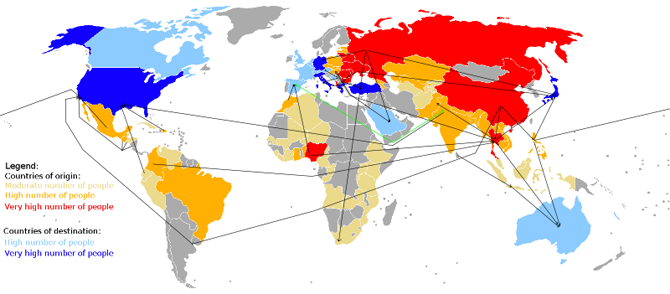
\includegraphics[width=6.5in,height=2.84722in]{image3.png}

\subsection{Vocabulary}

\begin{itemize}
\item 
\textbf{Branding}: A tattoo or carving on a victim that indicates
ownership by a trafficker/pimp/gang.
\item
\textbf{Circuit}: A series of cities among which prostituted people are
moved. One example would be the West Coast circuit of San Diego, Las
Vegas, Portland, and the cities in between. The term can also refer to a
chain of states such as the ``Minnesota pipeline'' by which victims are
moved through a series of locations from Minnesota to markets in New
York.
\item
\textbf{Coercion}: Threats or perceived threats of serious harm to or
physical constraints against any person; a scheme intended to cause a
person to believe that failure to perform will result in serious harm to
or physical restraint against any person.
\item
\textbf{Commercial Sex Act}: Any sex act on account of which anything of
value is given to or received by any person.
\item
\textbf{Exit Fee}: The money a pimp will demand from a victim who is
thinking about trying to leave. It will be an exorbitant sum, to
discourage her from leaving. Most pimps never let their victims leave
freely.
\item
\textbf{Facilitators}: It is important to realize that human trafficking
operations often intersect or exist alongside legitimate businesses. As
a result, certain industries may help to enable, support, or facilitate
human trafficking. This ``support structure'' may include a wide range
of individuals, organizations, businesses and corporations, and Internet
sites and practices. Common facilitators on which traffickers frequently
rely include:

\begin{itemize}
\item
  
  Hotels and Motels
  
\item
  
  Landlords
  
\item
  
  Labor brokers
  
\item
  
  Taxi and other driving services
  
\end{itemize}
\item
\textbf{Fraud}: Knowingly misrepresenting the truth or concealing an
actual fact for the purpose of inducing another person to act to her/his
detriment. Examples of fraud include false promises for specific
employment, being promised a certain amount of money that is never paid,
working conditions are not as promised, being told she or he would
receive legitimate immigration papers or a green card to work but the
documents are not obtained.
\item
\textbf{Human smuggling:} The facilitation, transportation, attempted
transportation, or illegal entry of a person or persons across an
international border, in violation of one or more countries' laws,
either clandestinely or through deception, such as the use of fraudulent
documents.
\item
\textbf{Quota}: A set amount of money that a trafficking victim must
make each night before she can come ``home.'' Quotas are often set
between \$300 and \$2000. If the victim returns without meeting the
quota, she is typically beaten and sent back out on the street to earn
the rest. Quotas vary according to geographic region, local events, etc.
\item
\textbf{Seasoning}: A combination of psychological manipulation,
intimidation, gang rape, sodomy, beatings, deprivation of food or sleep,
isolation from friends or family and other sources of support, and
threatening or holding hostage of a victim's children. Seasoning is
designed to break down a victim's resistance and ensure compliance.
\item
\textbf{Traffickers}: Traffickers are people who exploit others for
profit. They can be any demographic, individuals and groups, street
gangs and organized crime, businesses or contractors.
\item
\textbf{The Wire}: (1) A pimp hotline, like a phone tree pimps use to
get the word around, to find out which city is on/off. (2) Wiring money
from victim to pimp in different cities/states (``put it on the wire'').
\end{itemize}

\subsection{Questions to Consider}

\begin{itemize}
\item
  
  Are there any possible ways to warn potential victims of the dangers
  of trafficking, raise awareness and discourage demand?
  
\item
  
  Have any comprehensive national policies and programs been successful,
  and how can they continue to be improved?
  
\item
  
  How can police, prosecutors, and judges be trained in fighting
  trafficking?
  
\item
  
  What are methods of identifying victims in how will investigations be
  carried out to ensure safety for these victims?
  
\item
  
  With national sovereignty in mind, what are ways in which nations can
  work together and collaborate to end human trafficking?
  
\end{itemize}

\end{document}
